\documentclass[tikz,border=6pt]{standalone}
\usepackage{lmodern}\usepackage[T1]{fontenc}
\usetikzlibrary{arrows.meta,positioning,calc}
\begin{document}
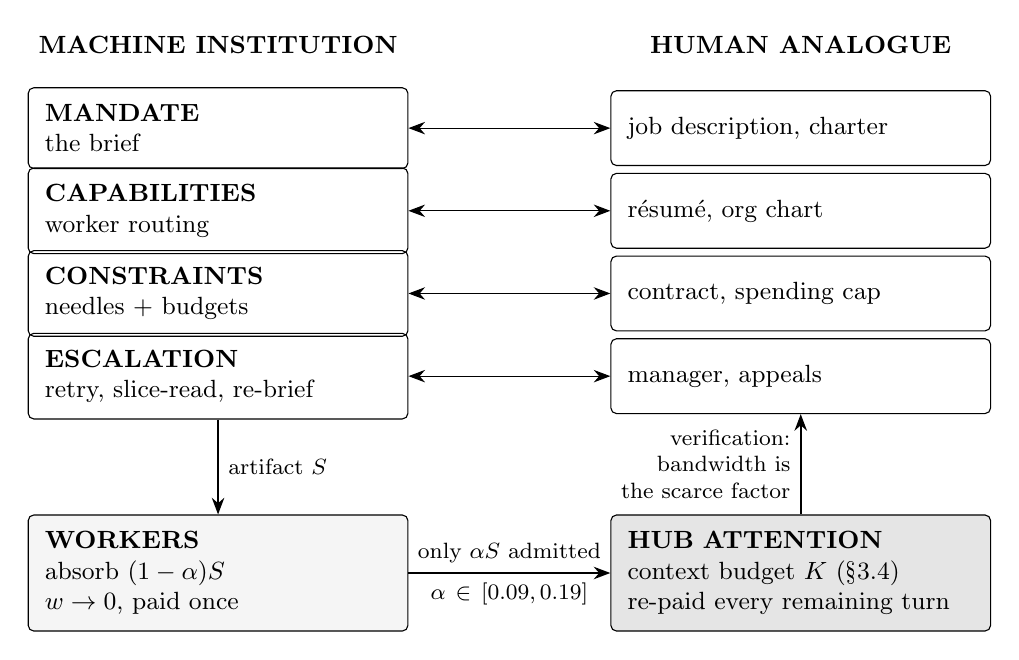
\begin{tikzpicture}[
  font=\small,
  every node/.style={align=left},
  >={Stealth[length=6pt]},
  box/.style={draw, rounded corners=2pt, inner sep=6pt, text width=4.4cm, minimum height=0.95cm},
]
% ---- top table: machine institution vs human analogue
\node[font=\small\bfseries] (hm) at (0,0) {MACHINE INSTITUTION};
\node[font=\small\bfseries] (hh) at (7.4,0) {HUMAN ANALOGUE};
\foreach \i/\L/\R/\M in {
  1/MANDATE/{the brief}/{job description, charter},
  2/CAPABILITIES/{worker routing}/{r\'esum\'e, org chart},
  3/CONSTRAINTS/{needles + budgets}/{contract, spending cap},
  4/ESCALATION/{retry, slice-read, re-brief}/{manager, appeals}} {
  \node[box] (m\i) at (0,-1.05*\i) {\textbf{\L}\\ \R};
  \node[box] (h\i) at (7.4,-1.05*\i) {\M};
  \draw[<->, thin] (m\i.east) -- (h\i.west);
}
% ---- bottom band: the cost law
\node[box, text width=4.4cm, fill=black!4] (workers) at (0,-6.7)
  {\textbf{WORKERS}\\ absorb $(1-\alpha)S$\\ $w \to 0$, paid once};
\node[box, text width=4.4cm, fill=black!10] (hub) at (7.4,-6.7)
  {\textbf{HUB ATTENTION}\\ context budget $K$ (\S 3.4)\\ re-paid every remaining turn};
\draw[->, thick] (m4.south) -- node[right, font=\footnotesize] {artifact $S$} (workers.north);
\draw[->, thick] (workers.east) -- node[above, font=\footnotesize, text width=2.6cm, align=center] {only $\alpha S$ admitted}
  node[below, font=\footnotesize, text width=2.6cm, align=center] {$\alpha \in [0.09, 0.19]$} (hub.west);
\draw[->, thick] (hub.north) -- node[left, font=\footnotesize, text width=3.2cm, align=right] {verification:\\ bandwidth is the scarce factor} (h4.south);
\end{tikzpicture}
\end{document}
